\documentclass[12pt,letterpaper]{hmcpset}
\usepackage[margin=1in]{geometry}
\usepackage{graphicx}
\usepackage{hyperref}

% info for header block in upper right hand corner
\name{Name: \underline{\hspace{4cm}}}
\class{Math 45: Section \underline{\hspace{1cm}}}
\assignment{Assignment 6}
\duedate{4/27/18}

\begin{document}

\begin{problem}
1. Consider the IVP:
\begin{center}
    $y'' + 0.5y' + 16y = 100 \text{sin} (t)$\\
    $y(0) = 0, y'(0) = 0$.
\end{center}
\begin{enumerate}
    \item[(a)] Solve the IVP. Identify the components of the solution corresponding to the forced response
of the system (a.k.a. periodic steady-state response), and the transient behavior
of the system.
    \item[(b)] Identify the natural frequency.
    \item[(c)] On a single pair of axes, plot all three graphs: (1) the solution of the IVP (2) its
steady-state component and (3) the transient component. (You may use technology).
Recall the steady state component is the particular solution to the forced ODE and the
transient component is the solution to the homogeneous ODE.
\end{enumerate}

\end{problem}
\newpage

\begin{problem}
2. A $m$ kg mass is suspended at the end of a (massless) rod with length $L$ meters. The other
end of the rod is fixed at a pivot point. This arrangement that leads to a simple pendulum
that swings in a plane.
\begin{center}
   $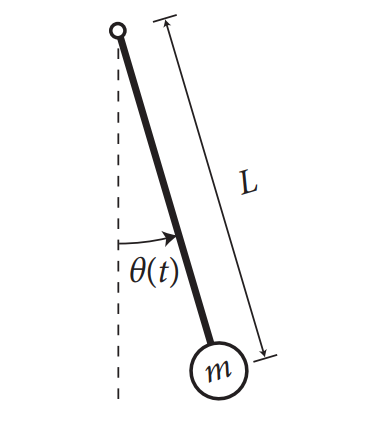
\includegraphics[scale=.4]{Pendulum.png}$ 
\end{center}
Suppose that there is no air resistance, friction, or any other mechanism that causes the
pendulum to lose energy. The only force acting on the pendulum is the force of gravity
pulling the mass down. Let $\theta(t)$ be the angular position of the pendulum, measured so that
the resting position of the pendulum corresponds to $\theta = 0$ and positive $\theta$ is in the direction of
the arrow above. In this problem, you will derive the governing equation of the pendulum’s
motion in two different ways.
\begin{enumerate}
    \item[(a)] First, you will derive a governing equation using the rotational analog of Newton’s
second law, $\tau = I \ddot{\theta}$. (You can consult your Physics 24 textbook for more information.)
You can assume that the mass is concentrated at a point and the rod is massless,
so the moment of inertia of the mass is $I = mL^2$
. Calculate the torque that results
from the force of gravity acting on the mass to obtain a differential equation for $\theta(t)$.
(You can consult your Physics 24 textbook for information about torque or \url{https://en.wikipedia.org/wiki/Torque}).
    \item[(b)] Now, you will rederive the same equation using conservation of energy. (You can consult
your Physics 24 textbook for more information). The total energy of the pendulum is
a sum of its potential and kinetic energy. Its kinetic energy is $\frac{1}{2}I\omega^2$, where $\omega = \dot{\theta}$ is the angular velocity of the mass about the pivot point. Calculate the potential energy
of the mass, relative to the lowest point that the mass can attain (at $\theta = 0$). Write down an expression for the total energy $E(t)$ of the pendulum, then take a derivative of
the $E(t)$, remembering to use the chain rule properly. Use the fact that the derivative
of $E(t)$ should be zero, since the total energy of the pendulum is constant, to derive a
differential equation for $\theta(t)$. After some algebraic simplification, you should arrive at
the same differential equation as in part (a).
\end{enumerate}

\end{problem}
\newpage


\begin{problem}
3. All higher order differential equations can be written as a system of first order DEs. Write
each of the DEs as a system of first order DEs. If the DE is linear, write the system in
matrix form (nonlinear DEs can not be put in matrix form). Note any restrictions on the
domain of the solution.

\begin{enumerate}
    \item[(a)] $4y'' - 11y' + 4y = 0$
    \item[(b)] 4$y'' - t^2y' + 4y = \text{sin} (t)$
    \item[(c)] $y^2y''' + 7y = 0$
\end{enumerate}

\end{problem}
\newpage

\begin{problem}
4. At $t = 0$ (i. e. noon) a student takes a fast-dissolving antihistamine capsule. The antihistamine
is absorbed from the GI tract (stomach and intestines) into the blood system and
then excreted. Let $x_1$ be the amount of antihistamine in the GI tract and $x_2$ be the amount
in the blood system. Assume that the rate of absorption from the GI tract into the blood
system is $k_1x_1$ and the rate of excretion from the bloodstream (via the kidneys) is $k_2x_2$,
corresponding to the following compartment diagram.
\begin{center}
   $\includegraphics[scale=.3]{compartment.png}$ 
\end{center}
\begin{enumerate}
    \item[(a)] Explain why the amount of antihistamine in the body satisfies the system
    \begin{center}
        $x'_1 = -k_1x_1$\\
        $x'_2 = k_1x_1 - k_2x_2$
    \end{center}
    together with the initial conditions $x_1(0) = \alpha$ and $x_2(0)=0$ where $\alpha$ is the initial
amount of antihistamine in the GI tract just after the capsule has dissolved.
    \item[(b)] Solve the system you found in part (a); you may assume that $k_2 < k_1$.\\
Hint: Note that you can solve the DE for $x_1$ first as it is independent of $x_2$.
    \item[(c)] When does the amount of antihistamine in the blood system reach a maximum? What
is the maximum amount? Your answers will be in terms of $\alpha$, $k_1$, and $k_2$ (Warning: the
exponential and logarithmic algebra may not be pretty, but please simplify as much as
you can).
\end{enumerate}

\end{problem}
\newpage

\begin{problem}
5. To solve a system of first order DEs with constant coefficients, we can use techniques related
to the characteristic equation and linear algebra. You will learn how to prove these results
in Math 65. Consider the linear system of DEs in matrix form for unknown functions $y(t)$
and $u(t)$:
\begin{center}
    $\frac{d}{dt}$\begin{bmatrix}
    y \\
    u
    \end{bmatrix}=
    \begin{bmatrix}
    1 & 2\\
    3 & 2
    \end{bmatrix}\begin{bmatrix}
    y \\
    u 
    \end{bmatrix}
\end{center}

\begin{enumerate}
    \item[(a)]Write the system in equation form (so you can see where the matrices came from).
    \item[(b)]Find the eigenvalues $\{ \lambda_1, \lambda_2\}$ and associated eigenvectors $\{ \Vec{v_1}, \Vec{v_2}\}$ of the matrix
    \begin{center}
        \begin{bmatrix}
    1 & 2\\
    3 & 2
    \end{bmatrix}
    \end{center}
    \item[(c)]Show that the solution
    \begin{center}
        \begin{bmatrix}
    y \\
    u
    \end{bmatrix}$=C_1\Vec{v_1}e^{\lambda_1t}+C_2\Vec{v_2}e^{\lambda_2t}$
    \end{center}
    solves the original system. Recall that to show that a
function is a solution you need to substitute it and its derivative into the system of
DEs.
    \item[(d)]Find $C_1$ and $C_2$ if the initial conditions for the system are:
    \begin{center}
        \begin{bmatrix}
    y(0) \\
    u(0) 
    \end{bmatrix}=
    \begin{bmatrix}
    1 \\
    -1 
    \end{bmatrix}
    \end{center}
\end{enumerate}

\end{problem}
\newpage

\begin{problem}
Review: Look back through HW 1–7, and the Midterm to remember what you found challenging.
Categorize what type(s) of errors/challenges you come across. Finally, come up with a plan
for how you’re going to address those errors/challenges before the Math 45 final exam
\end{problem}
% Add pairs of problems and solutions as needed

\end{document}
